\section{Lengde, Tid, og Tyngdeakselerasjon}

\subsection{Innledning}

Første eksperiment er delt i 3 forsøk, alle sentrert rundt lengde, tid, og usikkerheter. I første forsøk (Senere referert til som forsøk a) skulle vi måle perioden til et timeglass ved hjelp av stoppeklokke og pendel. I andre forsøk (Senere referert til som forsøk b) skulle vi måle forskjellige størrelser ved to klosser med tre forskjellige
måleinstrumenter. I tredje forsøk (Senere referert til som forsøk c) skulle vi estimere tyngdeakselerasjonen i Oslo, ved hjelp av Foucault-pendelen som står i fysikkbygget.

Formålet bak forsøkene var å bli kjent med hvordan man utfører et eksperiment, hvordan man dokumenterer dette, og bli introdusert til metoder for å estimere usikkerheter og propagere feil. Både lengde og tid er størrelser som introduserer usikkerheter, siden det ikke er mulig å måle dem helt presist. Det er dermed viktig å lære hvordan man kan, tross for disse usikkerhetene, måle så nøyaktig som mulig, og så kunne anslå akkurat hvor nøyaktig beregningene du har gjort er.

Disse forsøkene har også som formål å introdusere oss som studenter til hvordan det er å utføre et eksperiment rent praktisk. Hvor mange målinger man burde ta, hvordan man skal dokumentere prosessen underveis slik at man kan gjenskape det senere, og hvilke deler av eksperimentet man skal prioritere å få gjort, er viktig å lære, og dette første eksperimentet var en introduksjon til akkurat dette. 

\subsection{Material og Metoder}

Til forsøk a trengte vi en pendel for å måle svingninger (se fig 1), et timeglass vi skulle måle perioden av, stoppeklokker for å måle svingetid for pendelen og den totale tiden timeglasset brukte (I dette tilfellet brukte vi mobiltelefonene våre), og en meterstokk for å måle pendelens lengde.

Først tok vi mål av pendelens lengde, fra opphengspunkt til opphengspunkt. Så fant vi lengden av halve pendelmassen, og la disse to målene sammen for å finne lengden på hele pendelen (Vi propagerte også feilene for disse).

En av oss løftet pendelen vekk fra bunnpunktet, og slapp den slik at den begynte å svinge. Samtidig snudde en annen på gruppa timeglasset slik at den hvite siden pekte nedover, og vi startet stoppeklokkene våre. Vi gjorde hele denne prosessen to ganger.

Så, for å finne pendelens svingetid, løftet vi pendelen til samme punkt, og slapp den mens vi startet stoppeklokkene våre. Hver gang pendelen hadde svinget en hel periode, trykket vi på "runde" slik at vi lagret tiden for hele den nåværende perioden, uten at stoppeklokken stoppet å telle. Vi gjorde dette for 50 perioder. Vi sammenliknet våre mål med den teoretiske svingetiden, som vi fant ved:

\begin{align}
    T =2\pi\sqrt{\frac{L}{g}}\label{TFormula}
\end{align}

Der g = $9.82$ (gitt fra oppgavebeskrivelsen), og L er lengden vi har målt. Fra målingene våre plottet vi også histogram og regnet ut snitt og standardfeil i python.
\bigskip


Til forsøk b trengte vi målestokk, skyvelære, og lasermåler. Vi trengte også de to klossene vi skulle måle tykkelsen av (se fig 1), fra nå av referert til som kloss A og kloss B, der A er tykkere enn B.

Først skulle vi måle tykkelsen på begge klossene, ved hjelp av alle tre instrumentene. Vi tok mål så presist vi kunne, både ved oppsett av instrumentene og ved avlesning. Vi stilte opp målestokken inntil klossen vi skulle måle, og en av oss holdt den rett mens en annen leste av. Når vi skulle ta mål med skyvelæren, plasserte vi klossen i skyvelærens "klør" [DÅRLIG TERMINOLOGI], lukket den så tett på klossen som mulig, og leste av. Vi fant ut at lasermåleren har en grense på hvor korte distanser den kan måle, så vi kunne ikke måle klossens tykkelse direkte. Vi kom rundt dette ved å måle en lenger distanse, avstanden fra bunnen av bordet vi satt ved til gulvet, og så målte vi denne samme distansen etter vi hadde lagt klossen inn under laseren. Vi kunne da finne klossens tykkelse ved å se trekke det andre målet fra det første (dette introduserer enda en usikkerhet, som dokumenteres mer resultater-delen). Vi brukte de forskjellige målene våre for tykkelsene til kloss A og B, til å estimere differansen mellom tykkelsene deres.

\bigskip \hfil
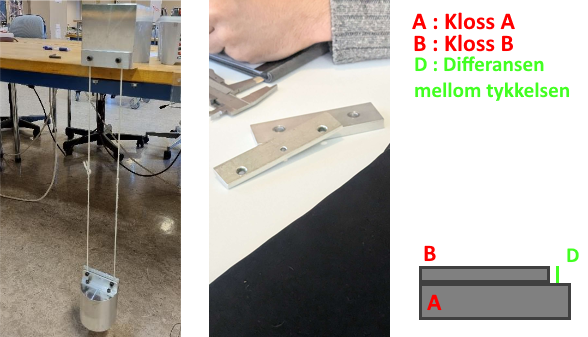
\includegraphics[scale = 0.8]{Figurer/Lab_Fig_1.png} 
\captionof{figure}{Pendel vi brukte i forsøk a (venstre), Klossene brukt i forsøk b (sentrum), og plassering av klossene i andre del av forsøk b (høyre).}
\par \bigskip

Så skulle vi måle differansen i tykkelse direkte, med målestokk og skyvelære. Vi stablet kloss B på toppen av kloss A (se fig 1), og tok mål. Med målestokken gjorde vi samme prosess som tidligere, mens med skyvelæren brukte vi "bunnen" [DÅRLIG TERMINOLOGI] til å måle differansen.\bigskip

Til forsøk c trengte vi lasermåleren, stoppeklokke (vi brukte igjen mobiltelefoner), Focault-pendelen som står i fysikkbygget, og diverse bøker av forskjellige størrelser.

Først målte vi tiden pendelen brukte på å svinge en hel periode, fra sentrum til sentrum. Vi gjorde dette alle tre, og fikk dermed 3 mål.

Så skulle vi finne lengden på pendelen. Vi stablet bøkene våre på toppen av hverandre, og plasserte lasermåleren på toppen av stabelen. Så pekte vi lasermåleren inn mot der pendelen når sitt laveste punkt. Så justerte vi høyden på stabelen fram til lasermåleren traff rett over pendelmassens midtpunkt (Vi ønsker å måle fra pendelmassens sentrum, men vi må ta lasermålerens tykkelse i betraktning. Derfor finner vi posisjonen litt over pendelmassens sentrum). Så snudde vi lasermåleren opp, for å måle distansen fra pendelmassens sentrum til taket. Til slutt, la vi til distansen mellom taket og der pendelen er hengt opp, som ble gitt i oppgaven.

Så estimerte vi vinkelens utslag, for å sjekke om småvinkelapproksimasjonen er gyldig. Vi tok et grovt mål fra den ene siden av gjerdet til den andre, og delte denne lengden i to (se fig 2). Vi kunne så finne tangens til det største vinkelutslaget ved å dele denne horisontale lengden på pendelens lengde, og så finne vinkelutslaget.

\hfil
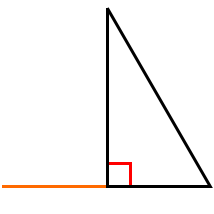
\includegraphics[scale = 0.8]{Figurer/Pendel_Lab1_c.png} 
\captionof{figure}{Lengder vi brukte til å anslå Foucault-pendelsens utslag. Her er summen av de to horisontale lengdene lik lengden fra den ene siden av gjerdet til den andre, mens den vertikale linjen er lengden på pendelen.}
\par \bigskip

Til slutt estimerte vi akselerasjonen i oslo ved bruk av uttrykket 

\begin{align}
    \hat{g} = \frac{4\pi^2l_p}{T^2}\label{ghat}
\end{align}

og sammenliknet det med $g = 9.82$, som vi vet er tyngdeakselerasjonen i oslo.
\bigskip

Til alle forsøkene brukte vi flere formler til å estimere feil, hovedsakelig

\begin{align}
    u_f = \sqrt{u_x^2 +u_y^2}\label{au}
\end{align}


som estimerer usikkerheten i summen av to usikre mål. Mer generelt anvendte vi 

\begin{align}
    u_f^2 = \left(\frac{\delta f}{\delta x} u_x\right)^2 + \left(\frac{\delta f}{\delta y} u_y\right)^2\label{gu}
\end{align}

for å estimere usikkerheter. Dersom et utrykk inneholder fler enn 2 variabler med usikkerheter, kan man da legge inn flere ledd i utrykket over.

\subsection{Resultater}

\subsubsection*{Forsøk a}

Vi fikk følgende mål for pendelens lengde:

\begin{center}
\begin{tabular}{ | c | c | c | }
    \hline
    & Lengde (cm) & Usikkerhet i avlesning (cm)\\ 
    \hline
    $l_o$ (mellom opphengspunkter) & 52.45 & 0.2\\ 
    \hline
    $l_m$ (pendelmassen) & 10.15 & 0.1\\ 
    \hline
\end{tabular}
\captionof{table}{Målinger av pendelens lengde}
\end{center}

for å estimere lengden av hele pendelen $l_p$, fra opphengspunkt til pendelmassens sentrum, må legge sammen $l_0$ og $\frac{l_m}{2}$. Dette gir oss $l_p = 62.6$. For å finne usikkerheten, bruker vi formel \ref{au}:

\begin{align}
    u_{l_p} = \sqrt{u_{l_o}^2 + u_{l_m}^2 + 2u_{ledd}^2 + 2u_{skala}^2}
\end{align}

her er $u_{ledd} = 0.5 \cdot 10^{-3} m$ og $u_{skala} = 0.5 \cdot 10^{-3} m$. Disse er usikkerhetene i målestokken, og ble gitt i oppgaveteksten. Dette gir oss 

\begin{align*}
    u_{l_p} &= \sqrt{\left(0.2\cdot10^{-2}\right)^2 + \left(0.1\cdot10^{-2}\right)^2 + \left(0.5\cdot10^{-3} \right)^2 + \left(0.5\cdot10^{-3} \right)^2} \; m\\
    &\approx 0.0023 \; \text{m}\\
    &= 0.23 \; \text{cm}
\end{align*}

Vi har altså $l_p = 62.6$ cm, og $u_{l_p} = 0.23$ cm. \bigskip

Som tidligere nevnt, målte vi timeglassets periode to ganger. Resultatet av disse målingene er som følger: 

\begin{center}
\begin{tabular}{ | c | c | c | }
    \hline
    & Første måling (sekunder) & Andre måling (sekunder)\\ 
    \hline
    Klokke 1 & 183.97 & 185.19 \\ 
    \hline
    Klokke 2 & 184.02 & 183.31\\ 
    \hline
    Klokke 3 & 183.94 & 183.91 \\ 
    \hline
\end{tabular}
\captionof{table}{Timeglassets periode målt med tre stoppeklokker}
\end{center}

\begin{center}
\begin{tabular}{ | c | c | c | }
    \hline
    & Første måling (antall) & Andre måling (antall)\\ 
    \hline
    Antall Svingninger & 122 & 120.5\\ 
    \hline
\end{tabular}
\captionof{table}{Timeglassets periode målt i antall perioder}
\end{center}

[SETT INN USIKKERHETER FOR DETTE HER!!!!] \bigskip

De 50 målingene tatt av pendelens svingetid ligger vedlagt i \nameref{Vedlegg}. Vedlagt ligger også program \ref{Svingehistogram.py}, som ble brukt til å plotte disse målingene. Dette produserte følgende histogram:

\begin{center}
    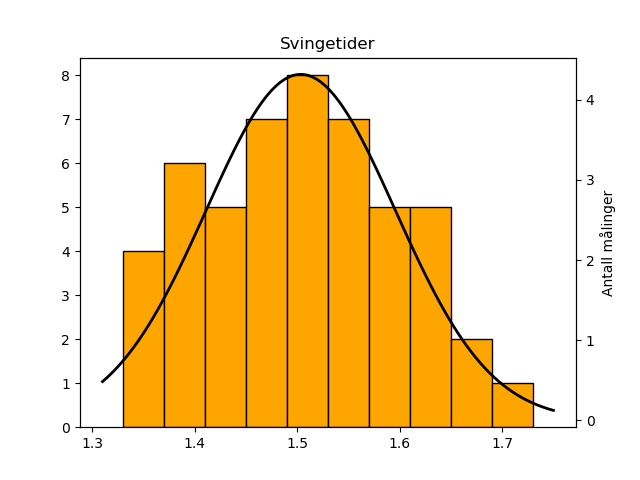
\includegraphics[scale = 0.6]{Figurer/Lab_1_Hist_1.png} \label{Hist_1}
    \captionof{figure}{Histogram av pendelens svingetider, sammen med den teoretiske normalfordelingen}
\end{center}

[KOMMENTER DETTE HER!!!]\bigskip

Fra programmet fikk vi også gjennomsnitt og standardfeil.

\begin{center}
\begin{tabular}{ | c | c | }
    \hline
    & Tid (sekunder)\\
    \hline
     $\bar{t}$ & 1.50\\
    \hline
     $SEM(t)$ & 0.0130\\
    \hline
\end{tabular}
\captionof{table}{Snitttid og standardfeil}
\end{center}

Vi kan sammelikne disse tallene med den teoretiske svingetiden vi får fra formel \ref{TFormula}, og så kan vi bruke formel \ref{gu} for å finne usikkerhetene.

\newcommand{\alignref}[1]{\;\;\;\text{$\left(\ref{#1}\right)$}}

\begin{align*}
    T =2\pi\sqrt{\frac{L}{g}} \alignref{TFormula}\\
    u_f^2 = \left(\frac{\delta f}{\delta x} u_x\right)^2 + \left(\frac{\delta f}{\delta y} u_y\right)^2 \alignref{gu}
\end{align*}

Dette gir oss

\begin{center}
\begin{tabular}{ | c | c | }
    \hline
    & Tid (sekunder)\\
    \hline
     $\accentset{*}{t}$ & 1.59\\
    \hline
     $u_{\accentset{*}{t}}$ & 0.0540\\
    \hline
\end{tabular}
\captionof{table}{Teoretisk tid og usikkerhet}
\end{center}

Vi kan så plotte denne teoretiske tiden sammen med histogrammet.

\begin{center}
    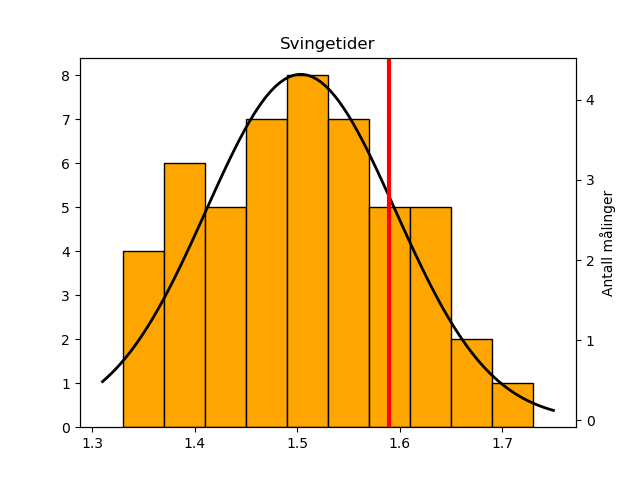
\includegraphics[scale = 0.6]{Figurer/Lab_1_Hist_2.png} \label{Hist_2}
    \captionof{figure}{Histogram av pendelens svingetider, sammen med den teoretiske normalfordelingen og den teoretiske svingetiden.}
\end{center}

\subsubsection*{Forsøk b}

Vi fikk følgende mål og usikkerheter for tykkelsene på klossene (Den totale usikkerheten er listet opp som $u_{total}$, som vi fant ved hjelp av formel \ref{au}):

\begin{center}
\begin{tabular}{ | c | c | c | c | c | c |}
    \hline
    & $l_a$ & $l_b$ & $u_{avles}$ & $u_{skala}$ & $u_{total}$\\
    \hline
     Skyvelære & 8.0  & 5.0  & 0.05 & 0.05 & 0.07\\
    \hline
     Målestokk & 8.0 & 5.0 & 0.5 & 0.5 & 0.9\\
     \hline
\end{tabular}
\captionof{table}{Mål og usikkerheter, gjort ved Skyvelære og målestokk, for tykkelsene på klossene (alt er målt i millimeter)}\label{table6}
\end{center}

\begin{center}
\begin{tabular}{ | c | c | c | c | c | c | c | c | c |}
    \hline
    & $l_t$ & $l_{t-a}$ & $l_{t-b}$ & $l_a$ & $l_b$ & $u_{avles}$ & $u_{skala}$ & $u_{total}$\\
    \hline
     Lasermåler & 719 & 709 & 713 & 10 & 6.0  & 0.0 & 2.0 & 2.8\\
    \hline
\end{tabular}
\captionof{table}{Mål og usikkerheter, gjort ved lasermåler, for tykkelsene på klossene (alt er målt i millimeter)}\label{table7}
\end{center}

I den totale usikkerheten til målestokken, måtte vi også ta med målestokkens $u_{ledd} = 0.5$mm, som ble gitt i oppgaveteksten.

Som nevnt var prosessen for å måle tykkelsene med lasermålet noe mer komplisert enn med de andre instrumentene. Vi måtte altså introdusere lengdene $l_t,l_{t-a}$, og $l_{t-b}$, som er lengdene fra bordet til gulvet, og fra bordet til gulvet etter vi hadde lagt klossene inn under laseren. Dette la til usikkerheter, som vi fant ved hjelp av formel \ref{au}.

\begin{align*}
    u_f = \sqrt{u_x^2 +u_y^2} \alignref{au}
\end{align*}

vi kan så finne $\Delta_{a-b}$ for alle målemetodene, og så, igjen ved hjelp av formel \ref{au}, finne usikkerhetene:

\begin{center}
\begin{tabular}{ | c | c | c |}
    \hline
    & $\Delta_{a-b}$ & $u_{\Delta_{a-b}}$\\
    \hline
     Skyvelære & 3.0 & 0.099\\
    \hline
     Målestokk & 3.0 & 1.3\\
     \hline
     Lasermåler & 4.0 & 4.0\\
     \hline
\end{tabular}
\captionof{table}{Estimerte differanser i tykkelse, med usikkerheter (i millimeter)}\label{table8}
\end{center}

Så sammmenlikner vi med de målte differansene $\Delta_{a-b}$:

\begin{center}
\begin{tabular}{ | c | c | c | c | c |}
    \hline
    & $\Delta_{a-b}$  & $u_{avles}$ & $u_{skala}$ & $u_{total}$\\
    \hline
     Skyvelære & 3.2  & 0.05  & 0.05 & 0.07\\
    \hline
     Målestokk & 3.0 & 0.5 & 0.5 & 0.9 \\
     \hline
\end{tabular}
\captionof{table}{Målte differanser i tykkelse, med usikkerheter, gjort ved Skyvelære og målestokk (i millimeter)}\label{table9}
\end{center}

\subsubsection*{Forsøk c}

Vi fikk følgende mål på pendelens periode:

\begin{center}
\begin{tabular}{ | c | c |}
    \hline
    & tid (sekunder)\\
    \hline
    Klokke 1 & 7.45\\
    \hline
    Klokke 2 & 7.54\\
    \hline
    Klokke 3 & 7.58\\
    \hline
\end{tabular}
\captionof{table}{Målte perioder for Foucault-pendelen}
\end{center}

 Senere vil vi bruke snittet av disse, $\overline{t} = 7.52$s til å beregne tyngdeakselerasjonen, sammen med $SEM(t) = 0.0314$s, som usikkerheten (Denne usikkerheten ble funnet via et lite program, som er lagt ved som vedlegg \ref{SEM.py})
\medskip

Så fikk vi følgende mål for pendelens høyde:

\begin{center}
\begin{tabular}{ | c | c | c |}
    \hline
    & Lengde (meter) & Usikkerhet (meter)\\
    \hline
    $l_t$ & 13.714 & 0.05\\
    \hline
    $l_f \; \text{(gitt i oppgaven)}$ & 0.64  & 0.08\\
    \hline
    $l_p = l_t + l_f$ & 14.354 & 0.094\\
    \hline
\end{tabular}
\captionof{table}{Målt lengde for Foucault-pendelen}
\end{center}

Når vi skulle sjekke om småvinkelapproksimasjonen gjelder, målte vi $l_x = 2.53$ meter fra en side av gjerdet rundt pendelen til den andre (Vi regner ikke med usikkerheter her.). Vi deler denne lengden på to, og kan da finne det teoretisk største vinkelutslaget:

\begin{align*}
    \theta &= arctan\left(\frac{\frac{l_x}{2}}{l_p}\right)\\
    &= arctan\left(\frac{1.265}{14.354}\right)\\
    &= 5.0363^{\circ}
\end{align*}

Pendelen vil aldri svinge helt ut til gjerdet, så vi vet at det ordentlige største vinkelutslaget vil være mindre enn dette. Som regel bruker man ca $10^{\circ}$ som grensen for småvinkelapproksimasjonen, så vi kan si med godt grunnlag at småvinkelapproksimasjonen gjelder.\bigskip

Til slutt, estimerer vi tyngdeakselerasjonen ved bruk av formel \ref{ghat}

\begin{align*}
    \hat{g} &= \frac{4\pi^2l_p}{\overline{t}^2} \alignref{ghat}\\
    &= \frac{4\pi^214.354}{7.52}\\
    &= 10.02
\end{align*}

Så finner vi usikkerheten ved bruk av formel \ref{gu}:

\begin{align*}
    u_f^2 = \left(\frac{\delta f}{\delta x} u_x\right)^2 + \left(\frac{\delta f}{\delta y} u_y\right)^2 \alignref{gu}
\end{align*}

\begin{align*}
    u_{\hat{g}}^2 &= \left(\frac{\delta \hat{g}}{\delta \overline{t}} u_{\overline{t}}\right)^2 + \left(\frac{\delta \hat{g}}{\delta l_p} u_{l_p}\right)^2\\
    &=  \left(\frac{-8\pi^2l_p}{\overline{t}^3} u_{\overline{t}}\right)^2 + \left(\frac{4\pi^2}{\overline{t}^2} u_{\overline{t}}\right)^2\\
    &= 0.0113\\
    u_{\hat{g}} &= \sqrt{0.0113}\\
    &= 0.106
\end{align*}

Dermed har vi at $\hat{g} = 10.02$ m/$s^2$, og $u_{\hat{g}} = 0.106$ m/$s^2$.

\subsection{Diskusjon}

Disse forsøkene var de første vi gjorde, og vi var relativt uerfarne når vi gjennomførte dem. Jeg mener at vi i løpet av forsøkene ble bedre på både hvordan utføre forsøkene rent praktisk, men også på hvordan vi skulle tenke rundt dem. \medskip

I forsøk a kan vi se at den teoretiske svingetiden er mindre sikker enn den empiriske. Siden vi kun har ett mål å gå på når vi estimerer den teoretiske svingetiden, gir det mening at denne er mindre sikker. På figur \ref{Hist_2} kan vi også se at det empiriske snittet er forskjøvet litt mot høyre (langs tidsaksen). Siden alle mål brukt i dette histogrammet er tatt av meg, antar jeg at det systematiske avviket kommer av menneskelige feil, altså at jeg konsekvent tar for korte målinger.\medskip

I forsøk b ser vi at Skyvelæren og Målestokken måler tykkelsen på klossene ganske nøyaktig, mens Lasermåleren er dårlig egnet til å måle så korte distanser. I tabell \ref{table7} kan vi se at Lasermåleren har hele 2.8 mm usikkerhet, som er mye sammenliknet med målestokkens 0.9 mm og skyvelærens 0.07 mm vi kan se i tabell \ref{table6}. Mye av denne usikkerheten kommer fra at vi måtte måle tykkelsen i flere steg når vi brukte lasermåleren, men dette viser igjen at lasermåleren ikke er best egnet til å måle så korte distanser.

For differansen mellom tykkelsene, ser vi at å måle direkte som regel gir et sikrere mål. I tabell \ref{table9} ser vi at målet tatt med målestokk samsvarer med estimatene i tabell \ref{table8}, men at det direkte målet er mindre usikkert. Det direkte målet med skyvelæren er også mer nøyaktig, men samsvarer ikke helt med estimatet. Siden alle andre mål peker mot 3.0 (hvis vi ser bort fra lasermålingen) antar jeg det er en feil i denne målingen, jeg vil tro en avlesingsfeil, og om jeg skulle utført forsøket igjen ville jeg forsøkt enda mer å ta nøyaktige mål.
Siden den direkte målingen har lavere usikkerheter, mener jeg at denne er den beste metoden for å finne differansen.\medskip

I forsøk c, brukte vi snitt og standardfeil når vi skulle regne med den målte tiden, selv om vi bare hadde tre målinger. Dersom jeg skulle gjort forsøket igjen, ville jeg tatt flere målinger av pendelens svingetid, for å få et mer nøyaktig mål. Vårt endelige estimat $\hat{g} = 10.02$ m/$s^2$, med usikkerheten $u_{\hat{g}} = 0.106$ m/$s^2$, er ikke veldig langt unna den ordentlige Gravitasjonsakselerasjonen i oslo, som er $9.82$ m/$s^2$. For å få et enda bedre estimat, kunne vi som tidligere nevnt tatt flere mål av svingetiden. Måten vi brukte til å estimere pendelens lengde var heller ikke den beste. Jeg er sikker på at det finnes en bedre måte å måle denne lengden på. \medskip

Generelt, mener jeg at målene vi tok var relativt gode, men at det definitivt er mulige forbedringer. Jeg tror at dersom vi fikk gjennomføre forsøkene igjen, med den erfaringen vi har nå, at vi kunne fått mer nøyaktige resultater.